
\documentclass[12pt]{article}
\usepackage{enumitem}
\usepackage{mathtools}
\usepackage{amsthm}
\usepackage{graphicx}
\graphicspath{ {images/} }
\begin{document}

\title{Assignment 2}
\author{Darwin Ding}
\maketitle

\section*{Exercise 1.8}
The probability of picking a marble out of the bag and getting red is 0.9, and we are looking for the probability that we sample 10 random marbles and get 1 or 0 red marbles.

The probability of getting 0 red marbles is $(.1)^{10} = 10^{-10}$, and the probability of getting 1 red marble is $(.1)^9 * .9 * 10$, because we pulled 9 green marbles (with probability .1) and 1 red marble (probability .9), and there were 10 ways to do that.

The probability of doing either of those things is the sum of those two probabilities is $\boldsymbol{9.1 * 10^{-9}}$

\section*{Exercise 1.9}
Using Hoeffding's Inequality, $\mu = .9$. Since we're looking for $v \le .1$, $\epsilon \ge .9 - .1 = .8$. By definition, also, $N = 10$.

\begin{gather*}
P[|v - \mu| \ge \epsilon] \le 2e^{-2\epsilon^{2}N}
\\ \le 2e^{-2 * .8^2 * 10}
\\ \le \boldsymbol{5.52 * 10^{-6}}
\end{gather*}

\section*{Exercise 1.10 (needs checking)}
\begin{enumerate}[label=(\alph*)]
	\item After running the experiment a single time, $\mu$ for $v_0$ = \textbf{0.3}, $\mu$ for $v_{rand}$ = \textbf{0.5} and $\mu$ for $v_{min}$ = \textbf{0}
	\item 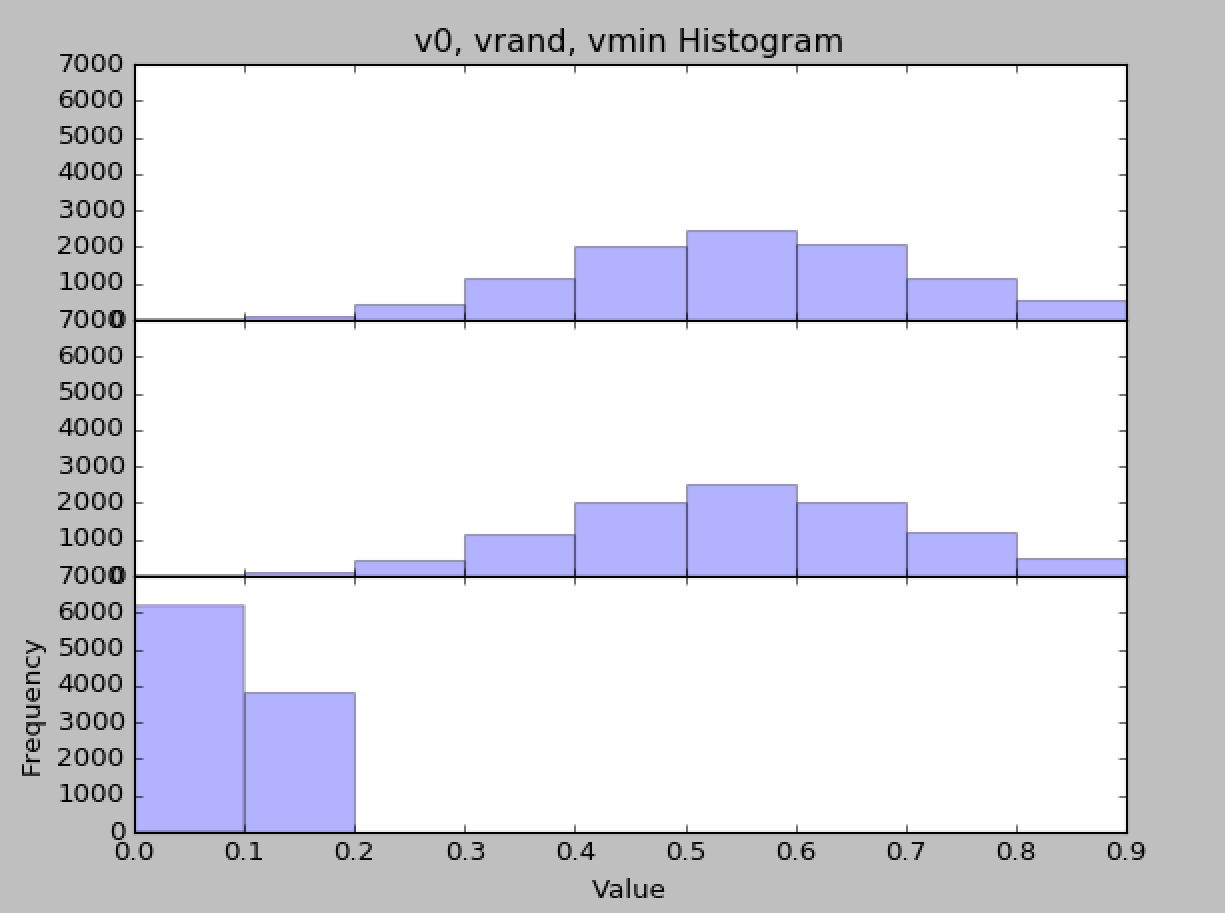
\includegraphics[scale=.5]{1-10-1.png}
	The top graph is of $v_0$, the middle graph is $v_{rand}$, and the bottom one is $v_{min}$.
	\item 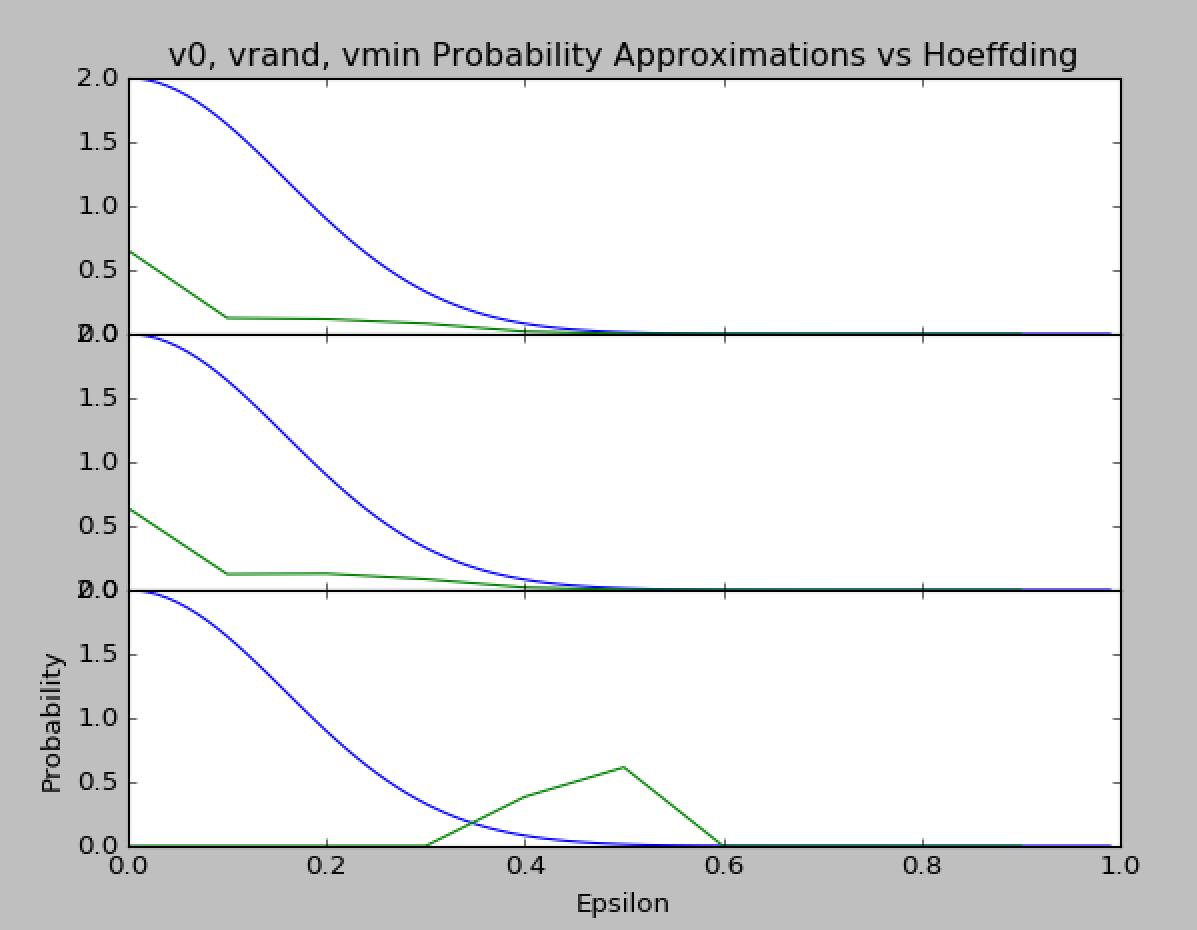
\includegraphics[scale=.5]{1-10-2.png}
	\item $v_0$ and $v_{rand}$ both obey the Hoeffding bound, while $v_{min}$ does not. This makes sense, because $v_0$ and $v_{rand}$ are essentially randomly selected coins. There's nothing special about the first coin or any random particular coin. The problem arises when you specifically seek out the minimum coin and then try to retroactively perform the Hoeffding bound. Hoeffding's inequality doesn't support this.
	\item If we pretend we don't know the true nature of coin flipping, and that $\mu$ is unknown to us, this problem is very similar to the bins problem. Let's say we are trying to predict $\mu$ using our data (the experiments we've performed and their results), and our hypothesis set is $[v_0, v_{rand}, v_{min}]$.
	\\ \\ If we fix our hypothesis set and then perform the experiment, we find that the Hoeffding bounds work simply because they work for $[v_0, v_{rand}]$. We cannot, however, claim that the bounds don't work simply because they retroactively don't work for $v_{min}$.
\end{enumerate}

\section*{Exercise 1.11 (check d)}
\begin{enumerate}[label=(\alph*)]
	\item No, not necessarily. If $p = 0.5$, then even if $E_{in}$ is approximately equal to $E_{out}$, $E_{in} = 0.5$ which is just as good as random.
	\item Yes. Just because the smart algorithm has the smallest in-sample error (even if it's 0) doesn't mean there's a chance that the out-of-sample data is completely different from the in-sample. In this case, all of the points out of D might be -1, and the crazy learning algorithm will have worked better.
	\item If $p = 0.9$, S will pick the "correct" hypothesis unless $E_{in}(h_1) > 0.5$. The probability of that is the probability that $\epsilon > .4$ ($E_{out}(h_1) = .1$). M = 2, so this probability is bounded by $2 * 2 * e^{-2\epsilon^2N}$ = .0013. Therefore the probability that S correctly hypothesizes from the set is at least 1 - .0013 = \textbf{0.99866}
	\item For any p, $E_in(h_1) = 1 - p$. Without loss of generality, let's assue that $p > 0.5$ (this could all be flipped and applied to the opposite case). $E_out(h_1)$ needs to be greater than 0.5 with probability greater than 0.5 for this to be true.
	\\ \\ Solving for $2 * 2 * e^{-2(p - 0.5)^2*25} > 0.5$ gets us \textbf{0.296 $<$ p $<$ 0.704}
\end{enumerate}

\section*{Exercise 1.12}
The best you can provide is \textbf{(c)}. Depending on the problem, you may need to have a very large hypothesis set, which would decrease your out-of-bound prediction accuracy. In that scenario, you may have to announce that you have failed. However, if you find that $E_{out}$ is not close to 0.5, then you can announce that you have found a function that approximates well out-of-sample.

\end{document}